

\usetikzlibrary{shadows,shapes.multipart}

\title{Arrays}
\author{Fr\'ed\'eric Vogels}


\begin{document}

\begin{frame}
  \titlepage
\end{frame}

\begin{frame}
  \frametitle{C-style Arrays}
  \begin{itemize}
    \item Syntactically resemble Java arrays
    \item Arrays in Java are evil
          \begin{itemize}
            \item Very rigid
            \item Use {\tt ArrayList} instead
          \end{itemize}
    \item Arrays in \cpp\ are even eviler
    \item Weird, complicated rules
    \item We'll focus on heap allocated arrays
    \item Couple of white lies for the sake of simplicity
  \end{itemize}
\end{frame}

\section{Arrays: The Sane Part}

\frame{\tableofcontents[currentsection]}

\begin{frame}
  \frametitle{What's an Array?}
  \code[language=c++14,width=.2\linewidth,frame=none]{array.cpp}
  \begin{center}
    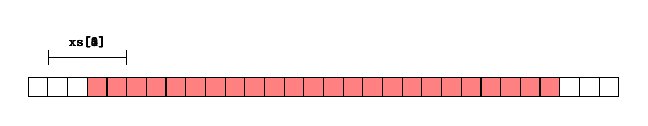
\begin{tikzpicture}[scale=.25]
      \draw[fill=red!50] (3,0) rectangle ++(24,1);

      \foreach \i in {0,...,5} {
        \tikzmath{
          int \x;
          \x = int(\i * 4 + 3);
        }

        \draw[|-|] (\x,2) -- ++(4,0) node[midway,above,font=\tiny] {\tt xs[\i]};
      }

      \draw (0,0) grid (30,1);
    \end{tikzpicture}
  \end{center}
  \begin{itemize}
    \item An array of \texttt{T}s is a series of consecutive \texttt{T}s in memory
    \item Indexing is zero based
  \end{itemize}
\end{frame}

\begin{frame}
  \frametitle{Type of Arrays}
  \code[language=c++14,width=.4\linewidth,frame=none]{array2.cpp}
  \begin{center}
    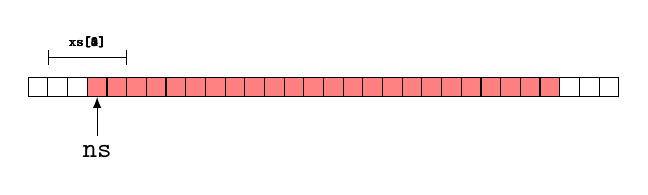
\begin{tikzpicture}[scale=.25]
      \draw[fill=red!50] (3,0) rectangle ++(24,1);

      \foreach \i in {0,...,5} {
        \tikzmath{
          int \x;
          \x = int(\i * 4 + 3);
        }

        \draw[|-|] (\x,2) -- ++(4,0) node[midway,above,font=\tiny] {\ttfamily xs[\i]};
      }

      \draw (0,0) grid (30,1);

      \draw[-latex] (3.5,0) ++(0,-2) -- ++(0,2) node[at start,below,font=\ttfamily] {ns};
    \end{tikzpicture}
  \end{center}
  \begin{itemize}
    \item An array of \texttt{T}s is written \texttt{T*}
    \item Is in fact a pointer pointing to first element
  \end{itemize}
\end{frame}

\begin{frame}
  \frametitle{Size of Arrays}
  \begin{itemize}
    \item You can't ask for an array's size
          \begin{itemize}
            \item You only know where the array starts
            \item But you don't get to know how many elements there are
          \end{itemize}
    \item If you need size, you'll have to keep track of it yourself
  \end{itemize}
\end{frame}

\begin{frame}
  \frametitle{Example of Security Vulnerability}
  \code[language=c++14]{vulnerability.cpp}
  \begin{itemize}
    \item Maximum input length allowed: 9
          \begin{itemize}
            \item If more, random memory gets overwritten
            \item Buffer overflow
            \item Very dangerous
          \end{itemize}
    \item Why 9, not 10?
          \begin{itemize}
            \item Strings must end with \texttt{0}
            \item Only true for strings!
          \end{itemize}
    \item Never use \texttt{char*} in \cpp, but \texttt{std::string}
  \end{itemize}
\end{frame}

\begin{frame}
  \frametitle{Freeing an Array}
  \code[language=c++14]{freeing.cpp}
  \begin{itemize}
    \item \texttt{delete p} only frees first element
          \begin{itemize}
            \item Memory leak!
          \end{itemize}
    \item \texttt{delete[] p} is necessary for arrays
          \begin{itemize}
            \item \texttt{delete[]} somehow knows the array's size
            \item But how it knows is secret!
            \item Must be stored somewhere
            \item Where is implementation dependent
          \end{itemize}
  \end{itemize}
\end{frame}

\begin{frame}
  \frametitle{Indexing}
  \code[language=c++14]{indexing.cpp}
  \begin{itemize}
    \item To access array elements, use \texttt{[]}
    \item But\dots array type is simple pointer!
    \item Is indistinguishable for single-element pointer
    \item How does \cpp\ know when to allow \texttt{[]}?
          \begin{itemize}
            \item \texttt{p[1]} should not be allowed
            \item \texttt{q[1]} should be allowed
          \end{itemize}
    \item Answer: \cpp\ does not know nor care
    \item You can use \texttt{[]} on \emph{all} pointers
  \end{itemize}
\end{frame}

\begin{frame}
  \frametitle{Indexing}
  \code[language=c++14]{indexing.cpp}
  \structure{Indexing on non-arrays}
  \begin{itemize}
    \item No difference between \texttt{*p} and \texttt{p[0]}, both ok
    \item \texttt{p[1]} reads beyond element
          \begin{itemize}
            \item Undefined behaviour
          \end{itemize}
  \end{itemize}
  \vskip5mm
  \structure{Indexing on arrays}
  \begin{itemize}
    \item Also no difference between \texttt{*q} and \texttt{q[0]}
    \item \texttt{q[1]} gives second element
  \end{itemize}
\end{frame}

\begin{frame}
  \frametitle{Indexing}
  \begin{itemize}
    \item Little difference between \texttt{new int} and \texttt{new int[1]}
    \item There's no separate array type in \cpp
    \item Indexing is allowed on all pointers
    \item No checks done
          \begin{itemize}
            \item Negative indices allowed (but undefined behaviour)
            \item Indexing beyond bounds also ok (but undefined behaviour)
          \end{itemize}
  \end{itemize}
\end{frame}

\begin{frame}
  \frametitle{Summary}
  \code[language=c++14,width=.6\linewidth]{summary.cpp}
\end{frame}

\section{Arrays: The Insane Part}

\frame{\tableofcontents[currentsection]}

\begin{frame}
  \frametitle{Stack Allocation}
  \code[language=c++14]{stack-allocation.cpp}
  \begin{itemize}
    \item You can allocate arrays on stack
    \item Size must be known at compile time
  \end{itemize}
\end{frame}

\begin{frame}
  \frametitle{Size}
  \code[language=c++14,font=\small,width=.95\linewidth]{sizeof.cpp}
  \begin{itemize}
    \item You can ask for the size of a stack allocated array
    \item But only in the same function that created it!
  \end{itemize}
\end{frame}

\begin{frame}
  \frametitle{Reason Behind Size Discrepancy}
  \structure{Bar}
  \begin{itemize}
    \item \texttt{bar} prints \texttt{20}
    \item \texttt{ns} has type \texttt{int[5]}
    \item Compiler can compute $5 \times 4 = 20$
  \end{itemize}
  \vskip5mm
  \structure{Foo}
  \begin{itemize}
    \item You cannot pass array types to functions!
    \item Type internally degrades to \texttt{int*} when calling \texttt{foo}
    \item \texttt{int*}, \texttt{int[]} or \texttt{int[5]} are identical parameter types
    \item \texttt{Foo} prints 4 because that is size of pointer
  \end{itemize}
\end{frame}

\section{What You Need To Know}

\frame{\tableofcontents[currentsection]}

\begin{frame}
  \frametitle{What You Need To Know}
  \begin{itemize}
    \item Only heap allocation
    \item Use \texttt{T*} as sole array type
    \item Assume size is always unknown
  \end{itemize}
\end{frame}

\end{document}


%%% Local Variables:
%%% mode: latex
%%% TeX-master: "arrays"
%%% End:
